

\documentclass[../../e1_tp1_main.tex]{subfiles}

\begin{document}

\newgeometry{left =2cm, right=2cm, top=2cm, bottom=2cm}

\chapter{}


En este ejercicio, se estudi\'o el comportamiento de un transistor NPN en el siguiente circuito con emisor com\'un:

\begin{figure}[H]

	\centering
 	\begin{circuitikz}
 	\draw 
 	(3.5,1) node[npn] (npn) {}
 
 	(npn.B) to [short, -*] (2.0,1)
 	to [C, l_=$C_{in}$, -*] (0.5,1) node[above]{$V_{in}$}
 	to [R, l_=$R_G$] (-1.5,1)
 	to [sinusoidal voltage source=$V_{G}$] (-1.5,-1.5) 
 	
 	(2,1) to [R, l_=$R_2$] (2.0,-1.5)
 	(2,1) to [R=$R_1$] (2.0, 3.5)
 	to [short] (-1.5,3.5)
 	to[american voltage source = $V_{CC}$] (-1.5,2) node[ground]{}
 	
 	(npn.E) to [R, l_= $R_E$] (3.5,-1.5)
 	(3.5,0.5) to [short, *-](5,0.5)
 	to [C, l_=$C_E$](5,-1.5)
 	
 	(npn.C) to [R, l_=$R_C$] (3.5,3.5)
 	to [short, -*] (2,3.5)
 	
 	(3.5,1.5) to [C=$C_{out}$, *-*] (6,1.5) node[right]{$V_{out}$}
 	to [R= $R_L$] (6,-1.5)
 	to [short, -*] (5,-1.5)
 	to [short, -*] (3.5,-1.5)
 	to [short] (-1.5,-1.5) node[ground]{}
 	
 	;\end{circuitikz}
 	
 	\caption{Esquema del circuito}
\end{figure}

En particular, el modelo de transistor utilizado fue el BC547\footnote{La hoja de datos de este transistor puede encontrarse en el siguiente link: \url{ https://www.sparkfun.com/datasheets/Components/BC546.pdf}}. Su $h_{fe}$, medido con mult\'imetro, es de 569.\par

Los valores de los componentes pasivos son los siguientes:


\begin{table}[H]
	\centering
	\begin{tabular}{|c|c|c|c|c|c|c|c|}
	\hline
	$R_1$        &	$R_2$	& $R_C$        & $R_E$       & $R_L$       & $C_{in}$ & $C_{out}$ & $C_{E}$  \\ \hline
	$100k\Omega$ & $8.2k\Omega$ & $5.6k\Omega$ & $250\Omega$ & 10$k\Omega$ & 10$nF$   & $10nF$    & $1\mu F$ \\ \hline
	\end{tabular}
	\caption{Valores de las resistencias y los capacitores utilizados}
\end{table}


La resistencia $R_G$ se encuentra excluida de estas consideraciones puesto a que es la resistencia interna del generador, cuyo valor est\'andar es $50\Omega$. A su vez, el transistor se aliment\'o con $V_{CC}=12V$ \par



\section{An\'alisis te\'orico}

A continuaci\'on obtendremos la respuesta para se\~nales de frecuencia media (donde los capacitores pueden considerarse cables) del circuito. Si bien con este m\'etodo no podremos obtener la respuesta en frecuencia del circuito, se espera que el valor m\'aximo de ganancia coincida con el calculado aqu\'i.

\subsection{Polarizaci\'on}
Como la polarizaci\'on del transistor se realiza en continua, no circula corriente por las ramas del circuito donde hay capacitores. Por lo tanto, se puede simplificar de la siguiente manera:

\begin{figure}[H]
	\centering
 	\begin{circuitikz}
 	\draw 
 	(3.5,1) node[npn] (npn) {}

 	(npn.B) to [short, -*] (2.0,1) 	
 	to [R, l_=$R_2$] (2.0,-1.5) node[ground]{}
 	
 	(2,1) to [R=$R_1$] (2.0, 3.5)
 	to [short] (-1.5,3.5)
 	to[american voltage source = $V_{CC}$] (-1.5,2) node[ground]{}
 	
 	(npn.E) to [R= $R_E$] (3.5,-1.5)
 	to [short, -*](2.0,-1.5)
 	
 	(npn.C) to [R, l_=$R_C$] (3.5,3.5)
 	to [short, -*] (2,3.5)
 	

 	;\end{circuitikz}
 	
 	\caption{Esquema del circuito en continua}
\end{figure}

Aplicaremos el teorema de Th\'evenin para resolverlo, es decir para obtener $I_{Cq} = h_{fe}\cdot I_{Bq}$. Aplicando un divisor resistivo obtenemos que $V_{Th} = \left( \frac{R_2}{R_1 + R_2} \right) \cdot V_{CC} = 0.909V$, con $R_{Th} =\frac{R_1 \cdot R_2}{R_1+R_2} = 7.579k\Omega$. Considerando que por la resistencia $R_E$ pasa $I_E=I_C+I_B=I_B\cdot(h_{FE}+1)$, el circuito resultante es entonces el siguiente:\par

\begin{figure}[H]
	\centering
	\label{fig:t2-thevenin}
 		\begin{circuitikz}
 		\draw 
	 	(3.5,1) node[npn] (npn) {}
 		(npn.B) to [R=$R_{Th}$] (-1,1)
 		to [american voltage source = $V_{Th}$] (-1,-1.5) node[ground]{}
 
 		(npn.E) to [R, l_= $R_E \cdot (1+h_{FE})$] (3.5,-1.5)
 		to [short, -*](-1,-1.5)
 		;\end{circuitikz}
 	\caption{Circuito de Th\'evenin en continua}
\end{figure}

De esta manera obtenemos que los valores de las corrientes de polarizaci\'on son:

	
 \[\left\{
\begin{aligned}
		I_{Bq} &=\frac{V_{Th}-V_{BE_{ON}}}{R_{Th} + R_E \cdot (1+h_{FE})} &= 1.467nA \\
		\\
		I_{Cq} &= h_{FE} \cdot I_{Bq} =  \frac{V_{Th}-V_{BE_{ON}}}{ \frac{R_{Th}}{h_{FE}} + R_E \cdot \left(\frac{1+h_{FE}}{h_{FE}}\right)} &= 835nA
 \end{aligned}
 \right.\]
 
 Con estas corrientes tan peque\~nas, la tensi\'on $V_{CE}$ es pr\'acticamente id\'entica a $V_{CC}=12V$, con lo cual estamos en el rango admitido por el fabricante para este par\'ametro (entre $45V$ de m\'aximo y $0.9V$ de saturaci\'on). En cuanto a la potencia, puesto que este transistor puede disipar hasta $500mW$ tampoco nos preocupa, y lo mismo con los $100mA$ m\'aximos para $I_C$. Por \'ultimo, siendo que la \textit{cut-off current} de este transistor es de $15nA$, se puede concluir que se est\'a trabajando en la \textit{safe operation area} para polarizaci\'on activa directa.
  
 
 	
\subsection{Modelo incremental}

Los par\'ametros que utilizaremos en el circuito incremental son los h\'ibridos. Para ello necesitaremos los valores de las tensiones $V_T$ y $V_A$. En cuanto a la primera, se considera que la misma vale $26mV$ pues se trabaja a temperatura ambiente. La tensi\'on de Early, por otro lado, la extrapolaremos de los gr\'aficos de $I_C(V_{CE})$ aportados por el fabricante.

\begin{figure} [H]
	\centering
	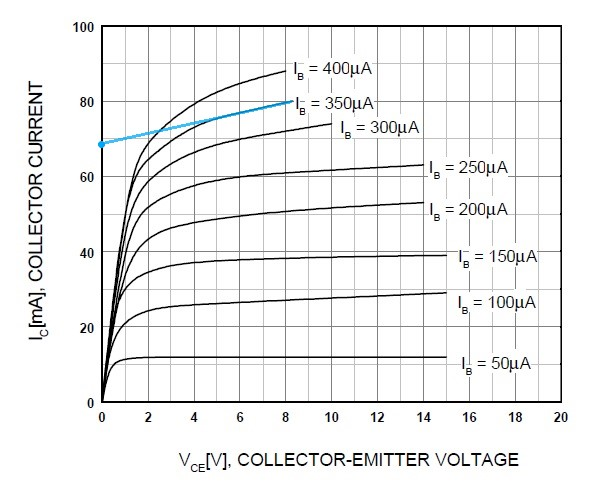
\includegraphics[scale=0.8]{imagenes/early.jpg}
	\caption{Curvas caracter\'isticas de la hoja de datos e interpolaci\'on lineal}
\end{figure}

La recta resaltada en celeste en la figura anterior intersecta al eje \textit{x} en $V_{CE}=-V_A$. Dado que su coordenada de origen es $I_{C0}\sim 68mA$, y su pendiente es $r_{ce}\sim \frac{8V}{80mA-68mA} = 667\Omega$, resulta que el valor de la tensi\'on de Early para este transistor es $V_A = r_{ce} \cdot I_{C0} \sim 45.33V$.\par

Habiendo determinado estos valores, los par\'ametros h\'ibridos resultan ser:

 \[\left\{
\begin{aligned}
	h_{ie}&= (h_{FE}+1) \cdot \frac{V_T}{I_{Cq}} &= 17.75M\Omega\\
	\frac{1}{h_{oe}} &= r_{oe} = \frac{V_A}{I_{Cq}} &= 54.29M\Omega
 \end{aligned}
 \right.\]


\subsection{Circuito incremental} \label{ssection:2-circuito-incremental}

Considerando que la frecuencia es lo suficientemente grande como para que la impedancia de los capacitores sea despreciable, el circuito queda planteado de la siguiente manera:

\begin{figure}[H]
	\centering
	\label{fig:circuito-incremental}
	\begin{circuitikz}
	\draw
	(0,2) to [sinusoidal voltage source = $V_{G}$] (0,0)
	(0,2) to [R = $R_G$] (2,2) node[above] {$V_{in}$}
	to [R = $R_{Th}$, *-*] (2,0)
	
	(2,2) to [short] (3.5,2)
	to [R = $h_{ie}$, -*, i>^=$i_b$] (3.5, 0)
	
	(6.5,2) to [dcisource,  l_= $h_{fe} \cdot i_b$] (6.5,0)
	to [short, *-*] (8,0)
	to [R, l_= $r_{oe}$, *-*] (8,2)
	(10,2) to [R=$R_C$, *-*] (10,0)
	
	(6.5,2) to [short, -*] (11.5,2) node[right]{$V_{out}$}
	to [R = $R_L$] (11.5,0)
	to [short] (0,0)

	;\end{circuitikz}
	
	\caption{Circuito en frecuencias medias, utilizando el modelo h\'ibrido para el transistor}
\end{figure}

Debido a que $r_{oe}\gg R_C\parsum R_L $, despreciamos sus efectos en el circuito. Las impedancias de este circuito son entonces:

\begin{equation}
	\label{eq:2-impedancias}
	\left\{
		\begin{aligned}
			R_D &= R_C\parsum R_L &= 3.590k\Omega\\
			R_{ia} &= R_{Th}\parsum h_{ie}  \sim R_{Th} &= 7.579k\Omega\\
			R_{oa} &= \frac{h_{fe} \cdot i_b \cdot R_C}{h_{fe} \cdot i_b}  = R_C &= 5.6k\Omega\\
		\end{aligned}
	\right.
\end{equation}

La ganancia en tensi\'on se obtiene entonces como:

\begin{equation}
	\label{eq:2-ganancia}
	\Delta_{V} = \frac{V_{out}}{V_{in}} = \frac{i_b \cdot h_{fe} \cdot R_D}{i_b\cdot R_{ia}} = \frac{h_{fe}\cdot R_D}{R_{ia}} = 270 = 49dB
\end{equation}

Si quisi\'esemos considerar la dependencia de la frecuencia para las impedancias de entrada y la salida, asumiendo que los valores de $h_{ie}$ y $r_{oe}$ siguen siendo lo suficientemente elevados como para que sean despreciables frente al resto de los valores, podr\'iamos agregar a este circuito los capacitores $C_{in}$ y $C_{out}$, que quedar\'an en serie respectivamente con $R_{Th}$ y $R_C$, resultando en dos circuitos pasa altos. La frecuencia de corte de estos circuitos ser\'ian entonces $f_{in} = \frac{1}{2\pi} \left(\frac{1}{R_{Th}C_{in}}\right) \sim 2.1kHz$ y $f_{out} = \frac{1}{2\pi} \left(\frac{1}{R_{C}C_{out}}\right) \sim 2.8kHz$



\section{Resultados y an\'alisis}

\subsection{Respuesta en frecuencia}


\begin{figure} [H]
	\centering
	\label{fig:2-hf}
	\begin{subfigure}[c]{\textwidth}
		\centering
		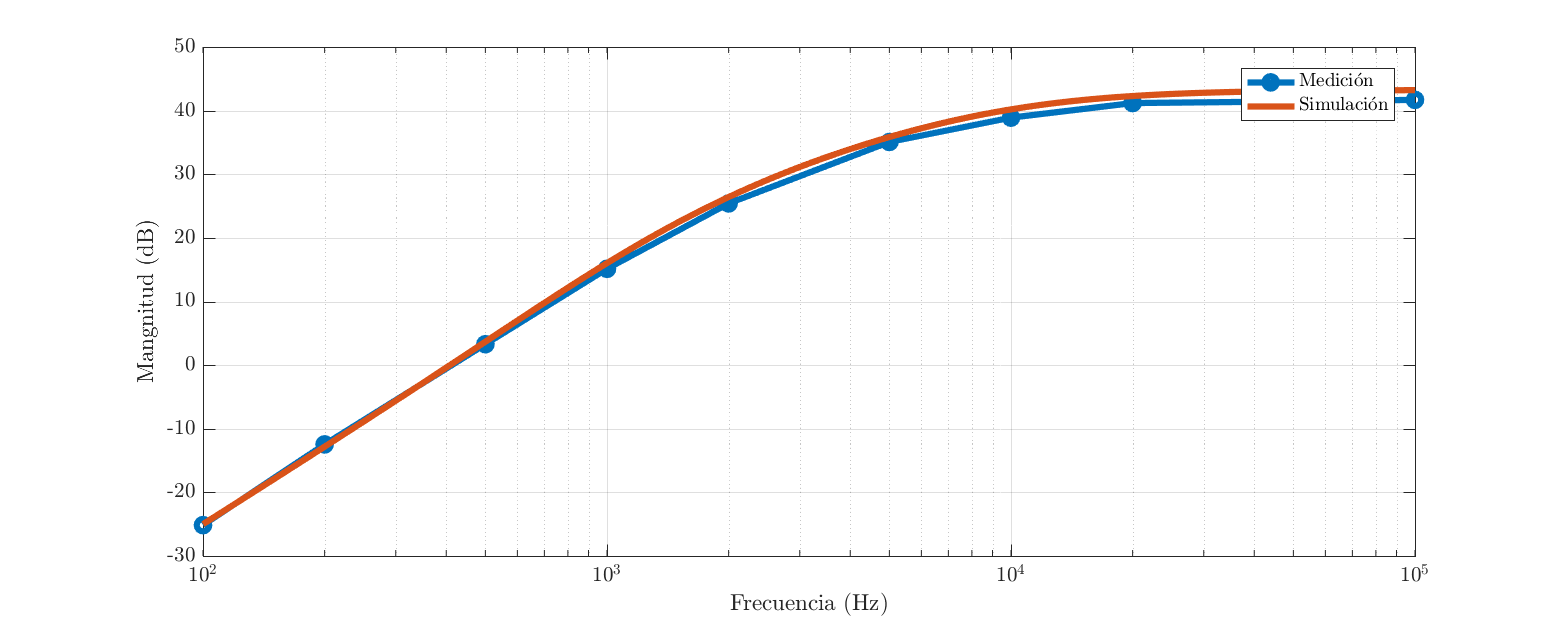
\includegraphics[scale=0.65]{imagenes/e1_tp1_ej2_hf_mag.png}
	\end{subfigure}
	
	
	\begin{subfigure}[c]{\textwidth}
		\centering
		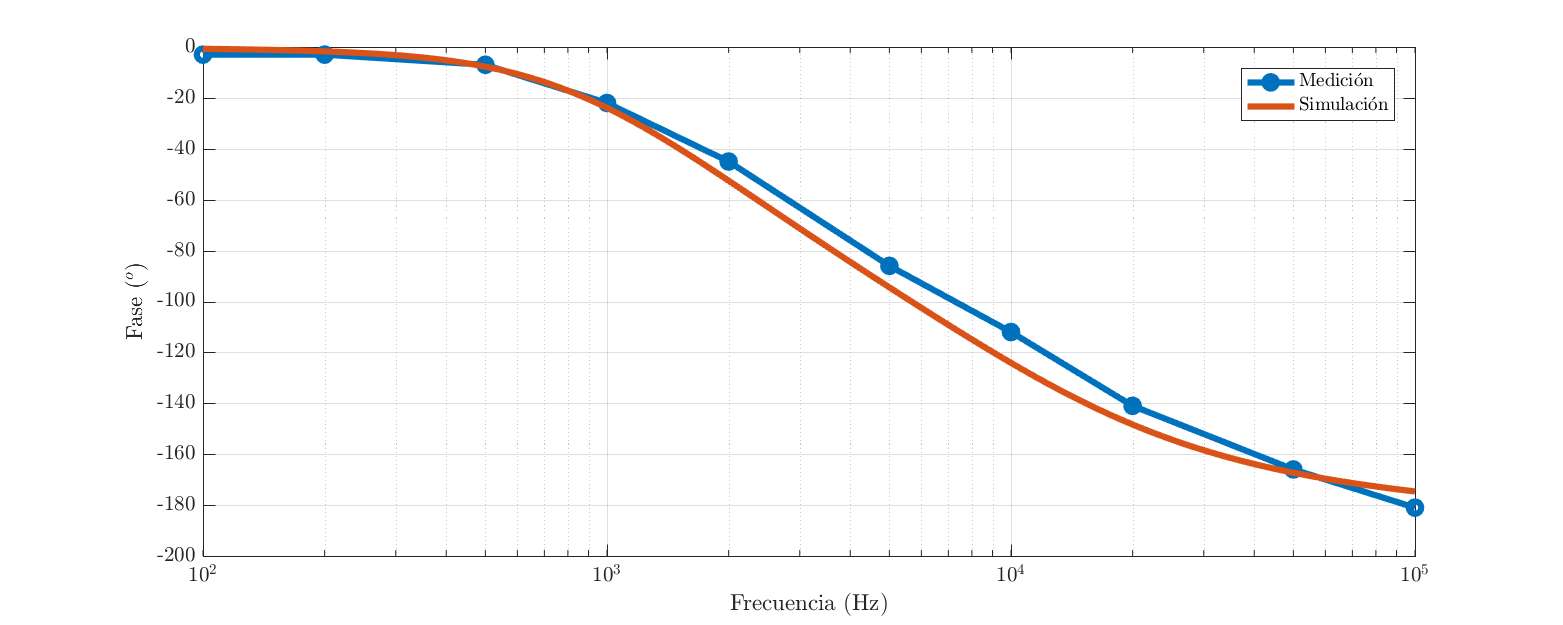
\includegraphics[scale=0.65]{imagenes/e1_tp1_ej2_hf_fase.png}
	\end{subfigure}
	
	\caption{Diagrama de bode de la respuesta en frecuencia}
\end{figure}

Las mediciones de ganancia en tensi\'on graficadas en la figura \ref{fig:2-hf} coinciden con lo simulado en \textit{LtSpice}. Se observa que inicialmente la ganancia crece $40dB$ por d\'ecada, y luego este crecimiento se ve limitado por un polo de segundo orden con $f_0 \sim 6k\Omega$ (donde la fase es aproximadamente $90^\circ$). As\'i para $f\gg 6k\Omega$, la ganancia se estabiliza en $42dB$. \par

Esto es considerablemente inferior a los $49dB$ obtenidos en la ecuaci\'on (\ref{eq:2-ganancia}). Esto podr\'ia deberse a que en esos c\'alculos se consider\'o que el valor de $h_{fe}$ era el mismo para continua que para frecuencias medias, y no necesariamente es este el caso. Asumiendo que la expresi\'on de $\Delta_V$ utilizada es v\'alida, las mediciones indicar\'ian que el valor de $h_{fe}$ en alterna es 338. Si este fuese el caso, las aproximaciones utilizadas para calcular las impedancias en (\ref{eq:2-impedancias}) a\'un pueden utilizarse, lo cual confirma que la expresi\'on de la ganancia se conserva. Considerando que la hoja de datos informa que $110 \leq h_{fe} \leq 800$, este resultado est\'a dentro de lo admitido por el fabricante.




\subsection{Impedancia de entrada}

\begin{figure} [H]
	\centering
	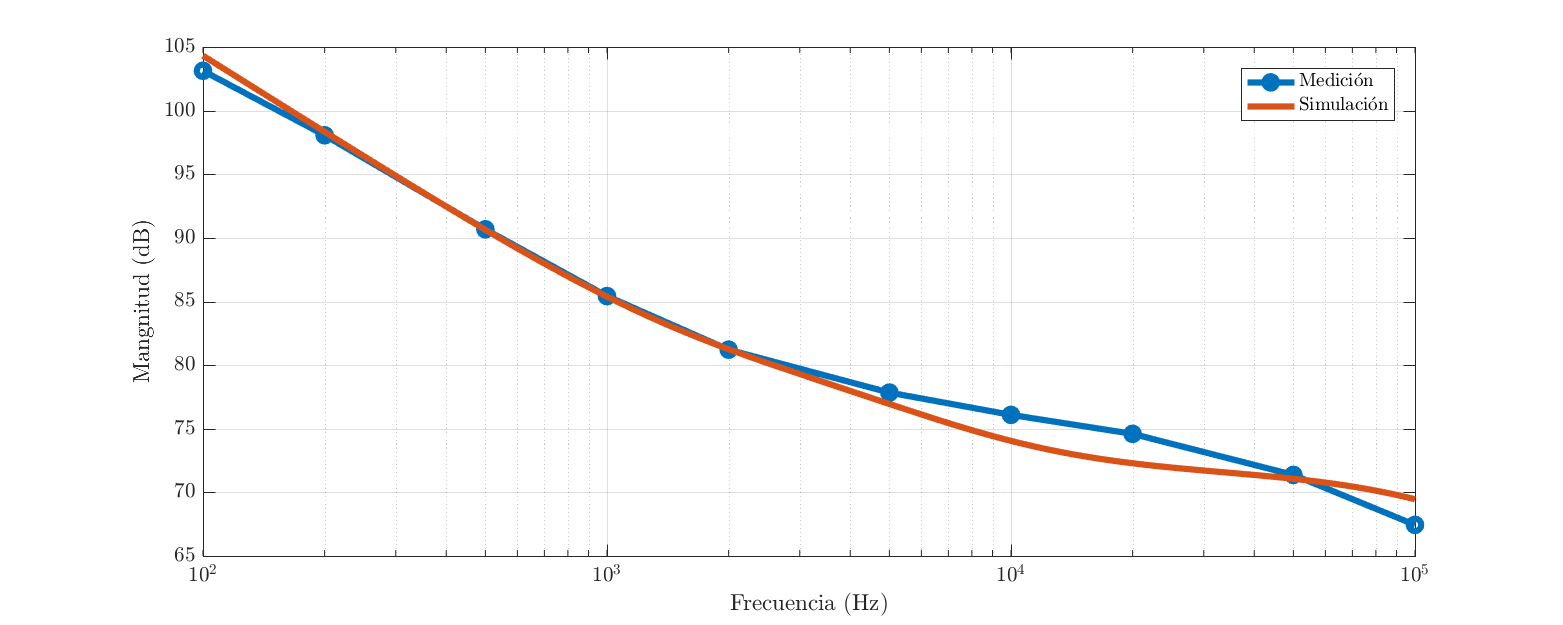
\includegraphics[scale=0.65]{imagenes/e1_tp1_ej2_zin_mag.png}	
	\caption{Diagrama de bode de la impedancia de entrada}
\end{figure}

Las mediciones pr\'acticamente coinciden con la simulaci\'on en el rango de frecuencias medido dentro de un margen de error aceptable. Sin embargo, este comportamiento no es el calculado en la secci\'on (\ref{ssection:2-circuito-incremental}), seg\'un lo cual la impedancia deber\'ia estabilizarse aproximadamente en $77dB$ para $f\gg 2kHz$. El modelo f\'isico utilizado, entonces, no es v\'alido para esta impedancia.



\subsection{Impedancia de salida}


\begin{figure} [H]
	\centering
	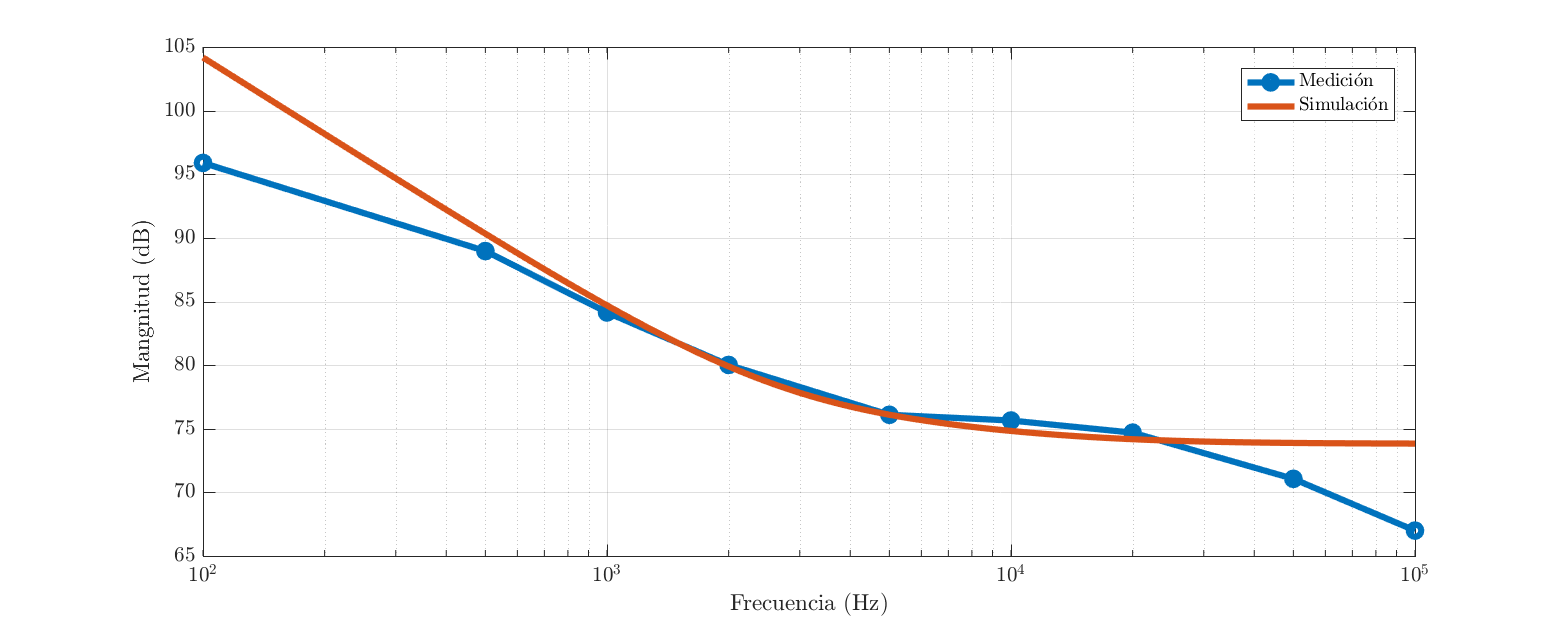
\includegraphics[scale=0.65]{imagenes/e1_tp1_ej2_zout_mag.png}	
	\caption{Diagrama de bode de la impedancia de entrada}
\end{figure}

En este caso, la simulaci\'on y las mediciones coinciden en el rango de frecuencias entre aproximadamente $5kHz$ y $200kHz$. A su vez, el valor en que la simulaci\'on predice que la impedancia es $75dB \sim 5.6k\Omega$, que se condice con el valor de $R_{oa}$ que hab\'iamos calculado en  (\ref{eq:2-impedancias}). Tambi\'en la frecuencia del polo est\'a en l\'inea con la calculada en la secci\'on (\ref{ssection:2-circuito-incremental}). En frecuencias m\'as altas, puede que efectos de inductancias par\'asitas, as\'i como las puntas del osciloscopio, est\'en interfiriendo en la medici\'on. Asimismo, puede haber discrepancias entre el modelo de \textit{spice} y el transistor utilizado que se manifiesten en este caso.



\section{Conclusiones}

Las mediciones efectuadas mayormente coincidieron con los c\'alculos de \textit{LtSpice}. Sin embargo, con el an\'alisis incremental s\'olo pudo predecirse adecuadamente el comportamiento de la impedancia de salida de acuerdo al simulador. Sin embargo, considerando que el valor de $h_{fe}$ no es el mismo para alterna que para continua, es posible explicar la ganancia en tensi\'on en frecuencias medias con este modelo, si bien no se cuenta con su valor para alterna y s\'olo podemos afirmar que seg\'un el modelo planteado, deber\'ia ser aproximadamente $338$. 

\end{document}

